\newpage
\section{Hundredths Grids for Rational Numbers}\label{A:hundredthsGrids}

%% Use tikz to generate the graphics

When a $10\times 10$ square is taken to be $1$ whole, it can be used as a ``hundredths grid'' 
to represent fractions and decimals between $0$ and $1$.\margincomment{For example, one of the grids below 
is shaded to represent $\frac{21}{100}$.}

\begin{prob}
Shade the hundredths grids to show each of the following fractions.  Then use your shading to determine a decimal equivalent for each fraction.  
\begin{center}
\hfill (a) $\frac{3}{20}$ \hfill (b) $\frac{1}{8}$ \hfill (c) $\frac{1}{6}$ \hfill (d) $\frac{7}{12}$ \hfill
\end{center}

\begin{fullwidth}\em\em\quad
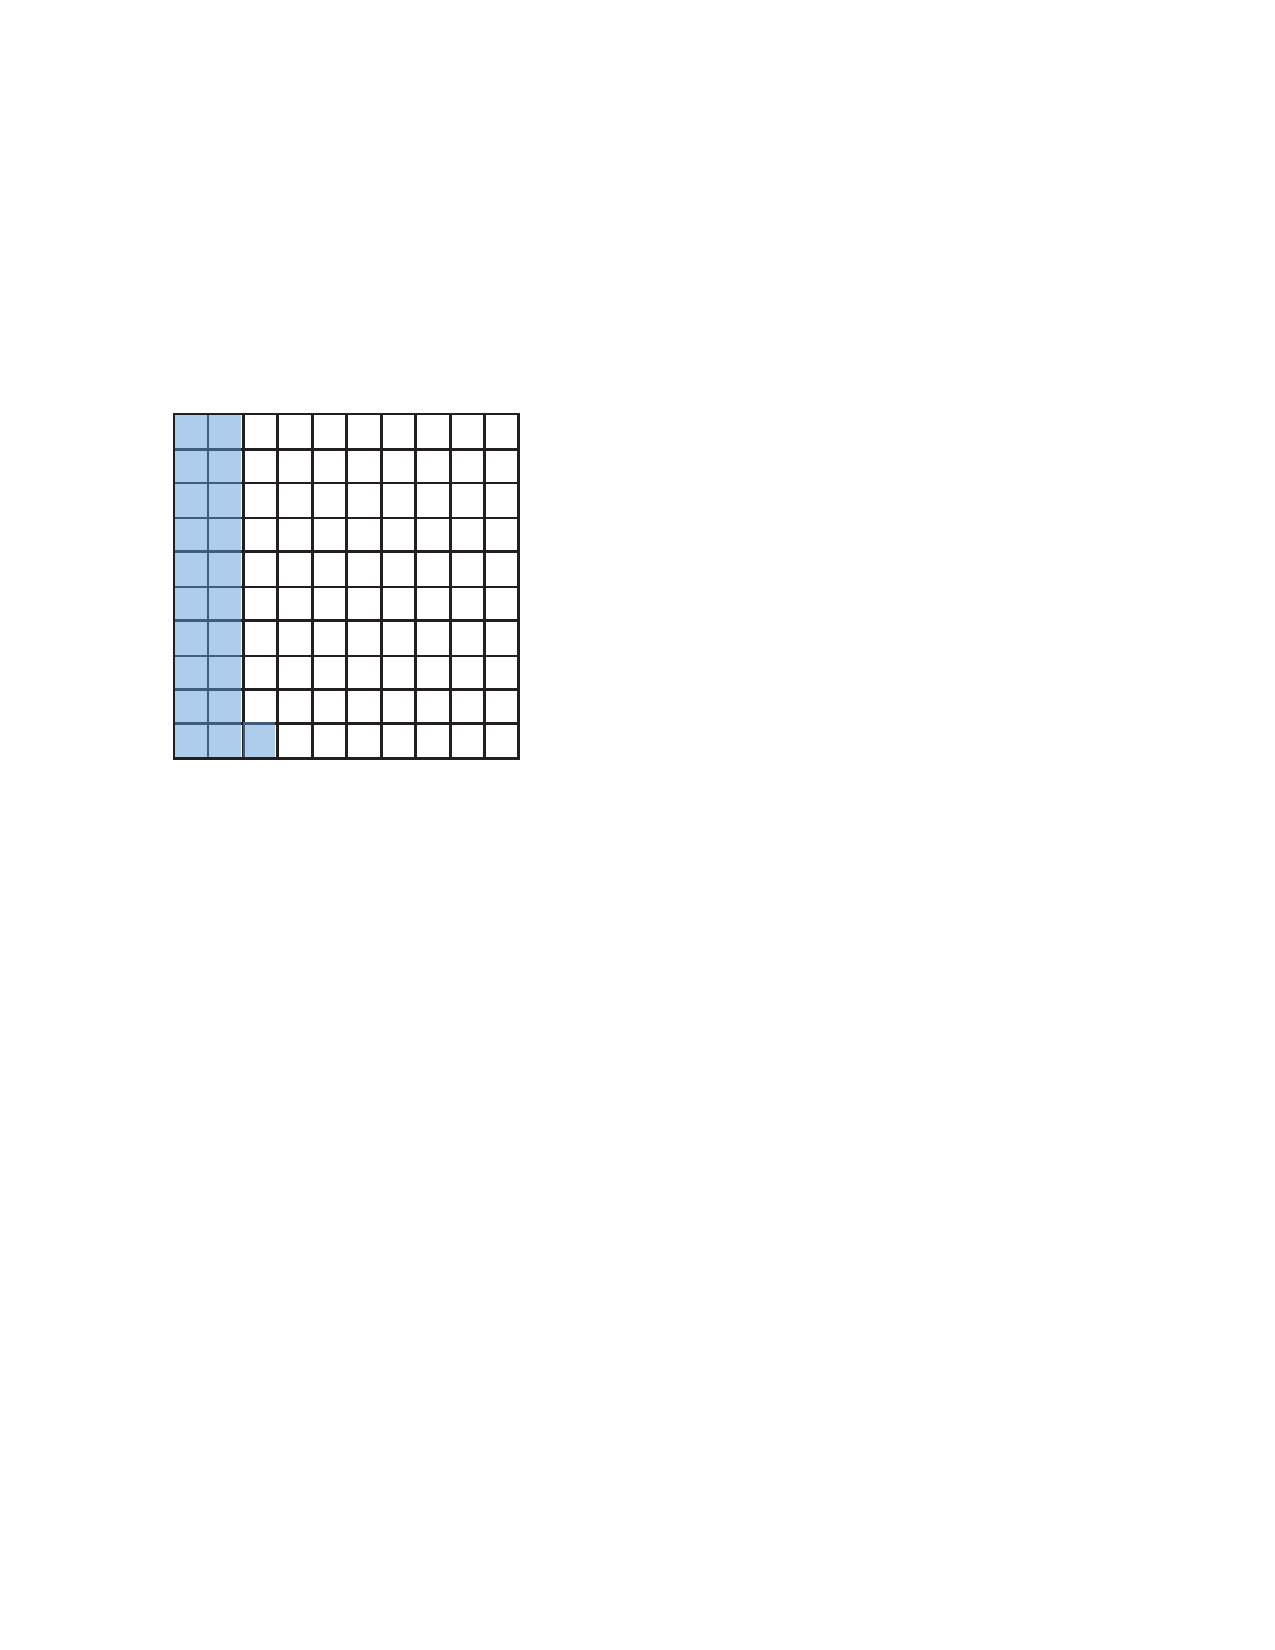
\includegraphics{../graphics/hundredthsGridSample}\quad
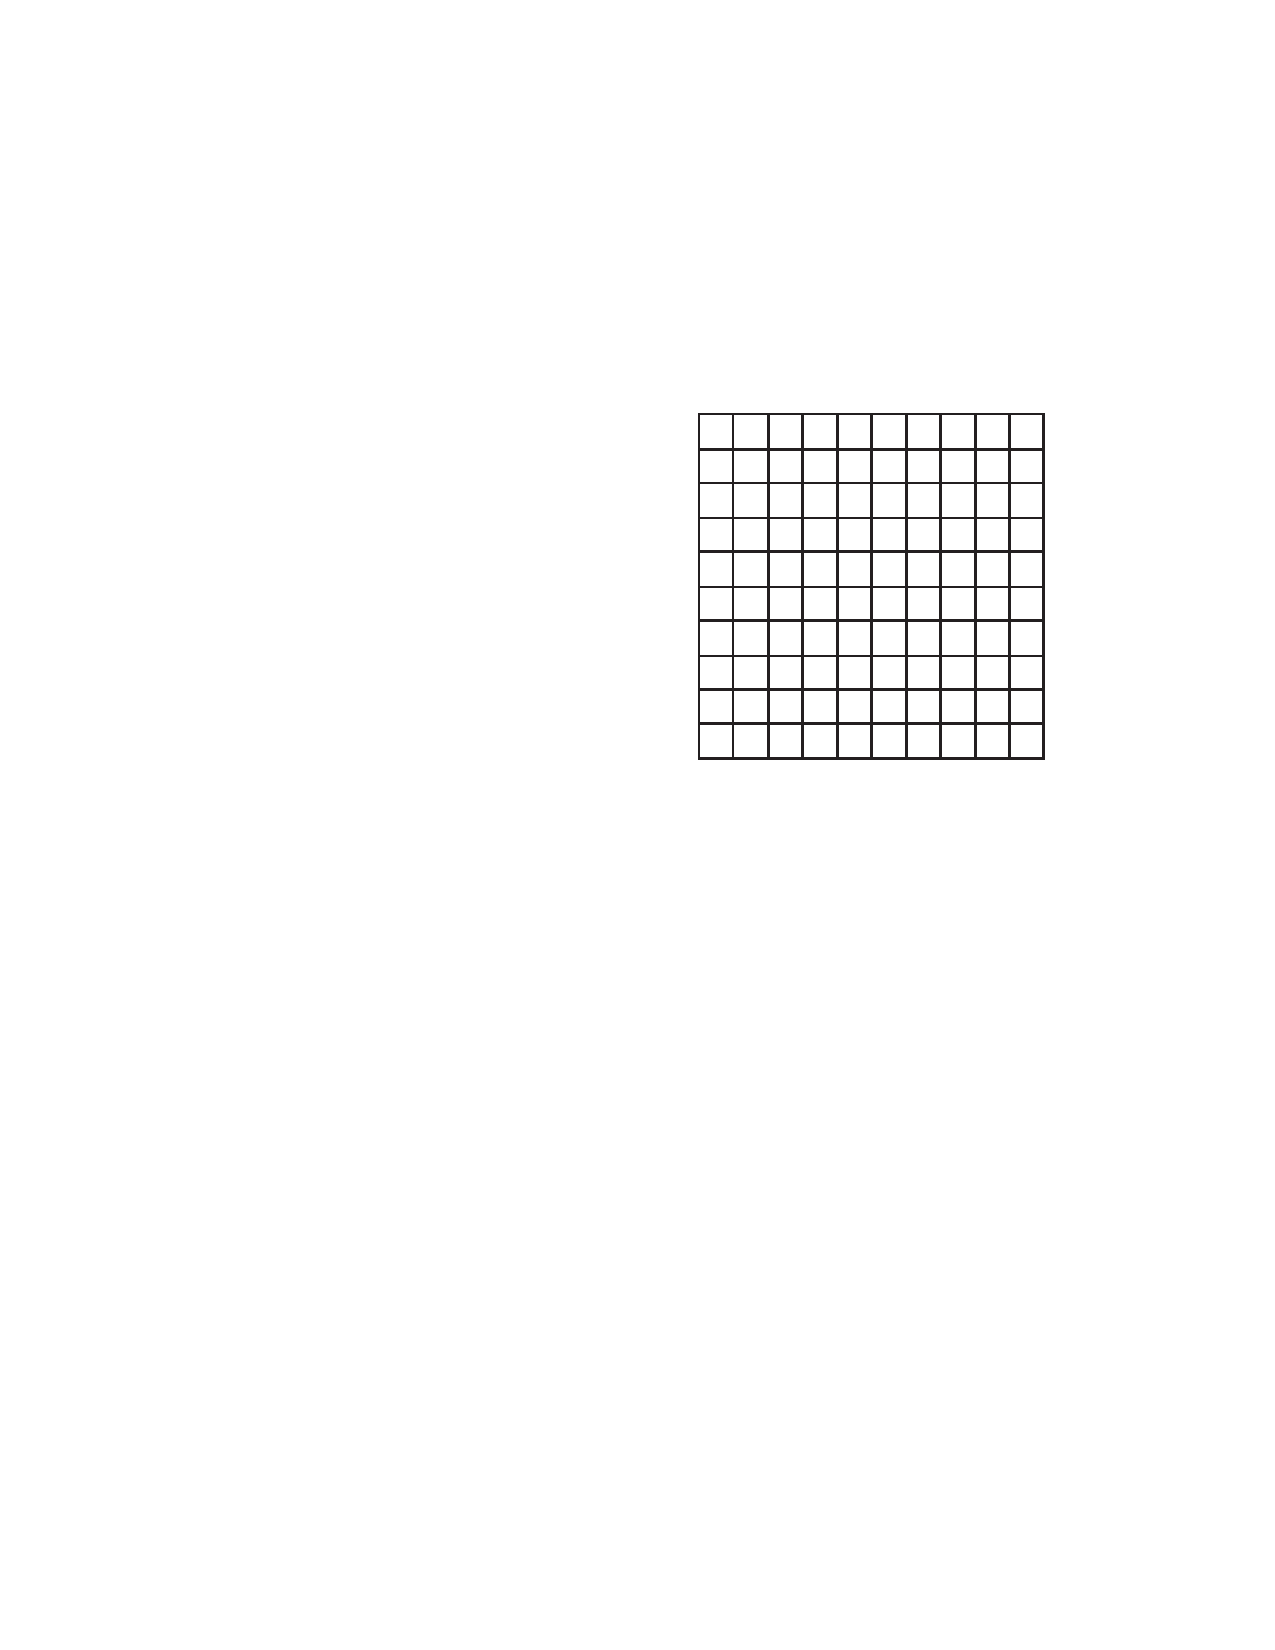
\includegraphics{../graphics/hundredthsGrid}\quad
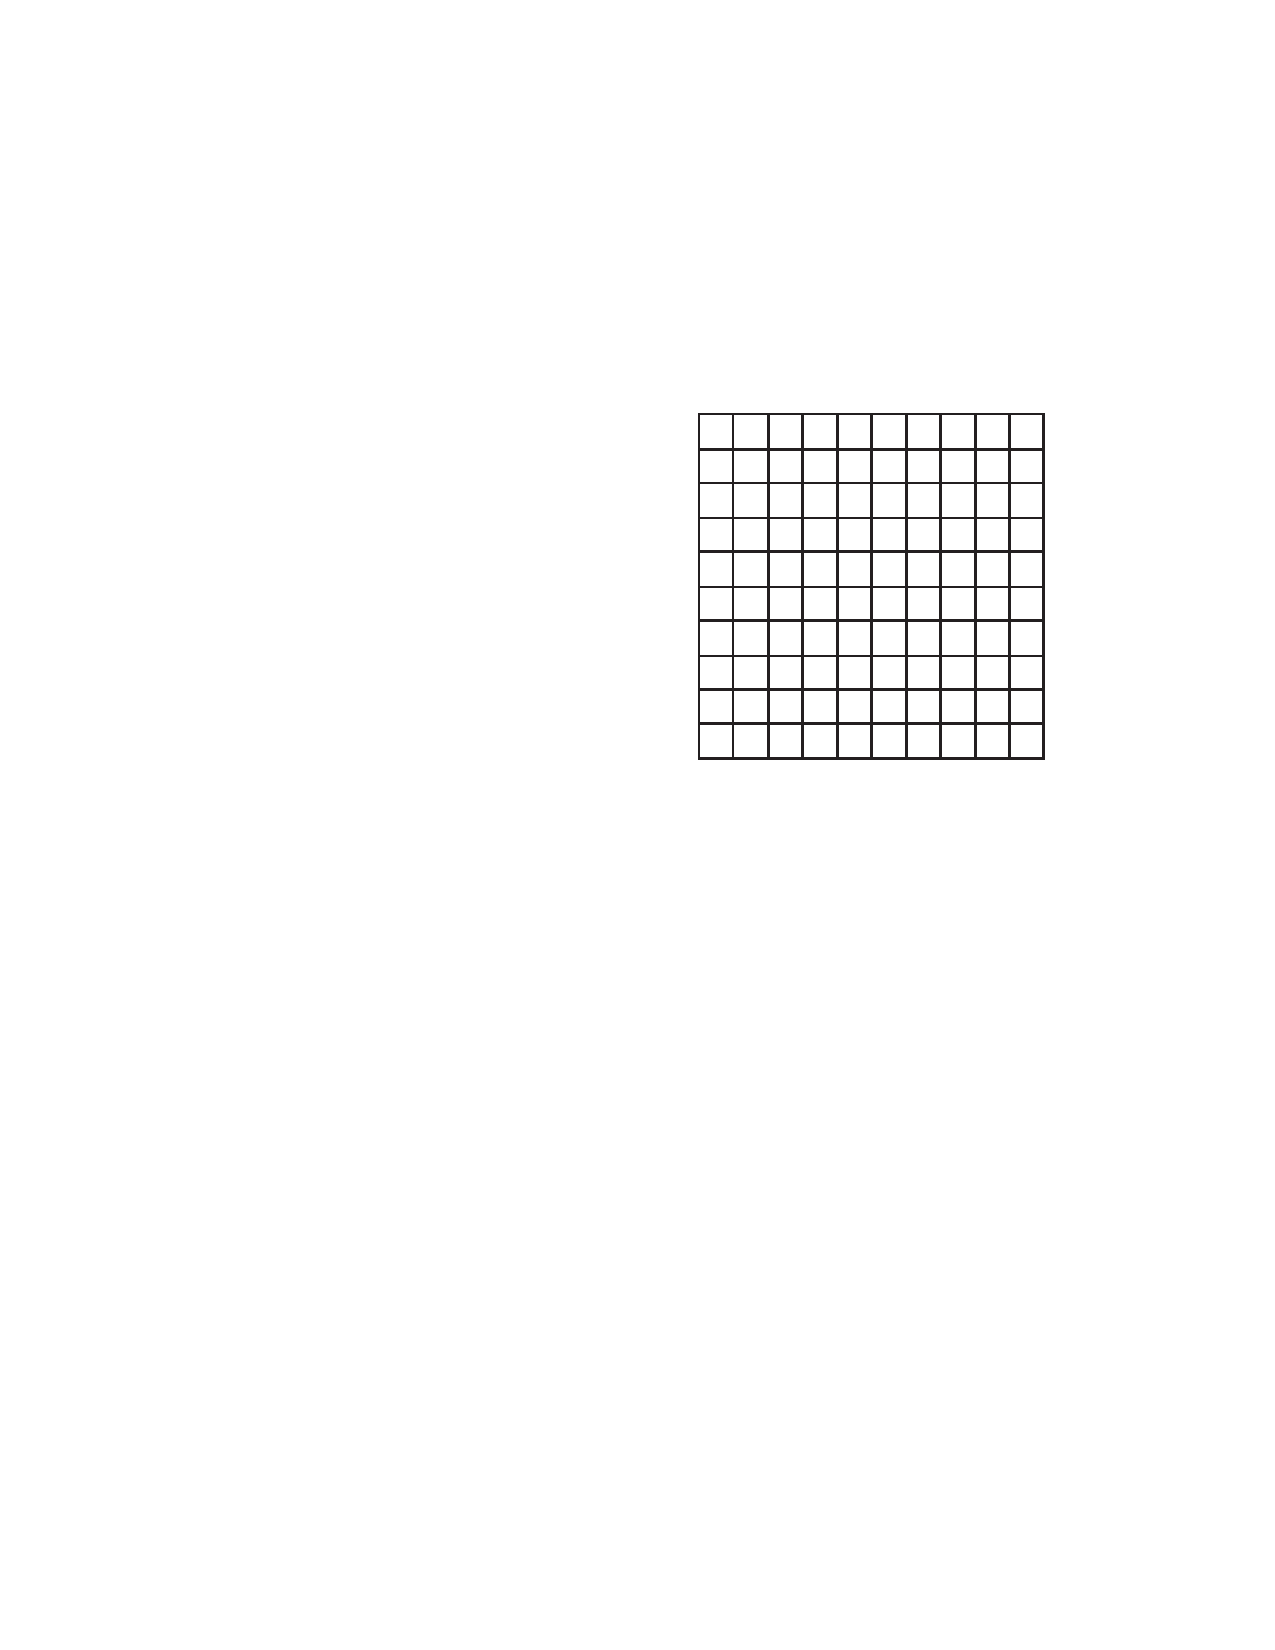
\includegraphics{../graphics/hundredthsGrid}\\

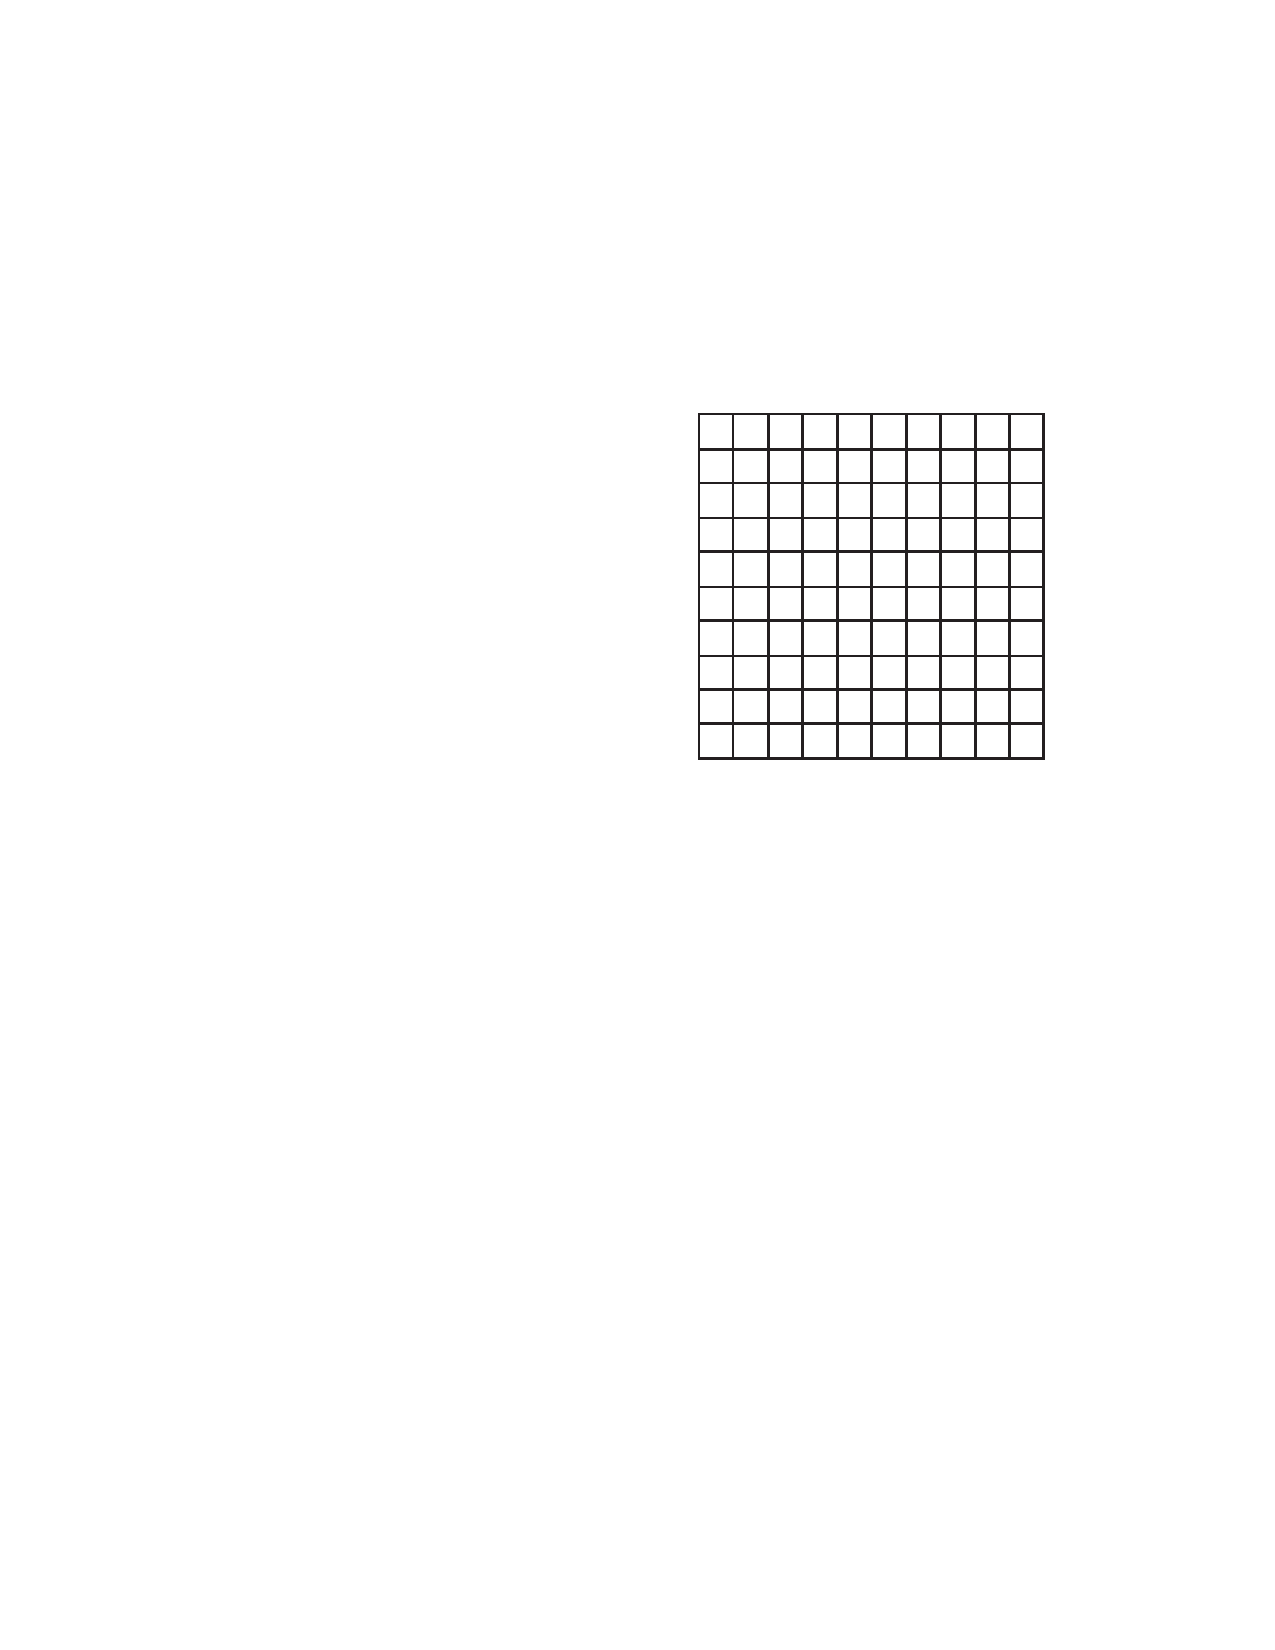
\includegraphics{../graphics/hundredthsGrid}\quad
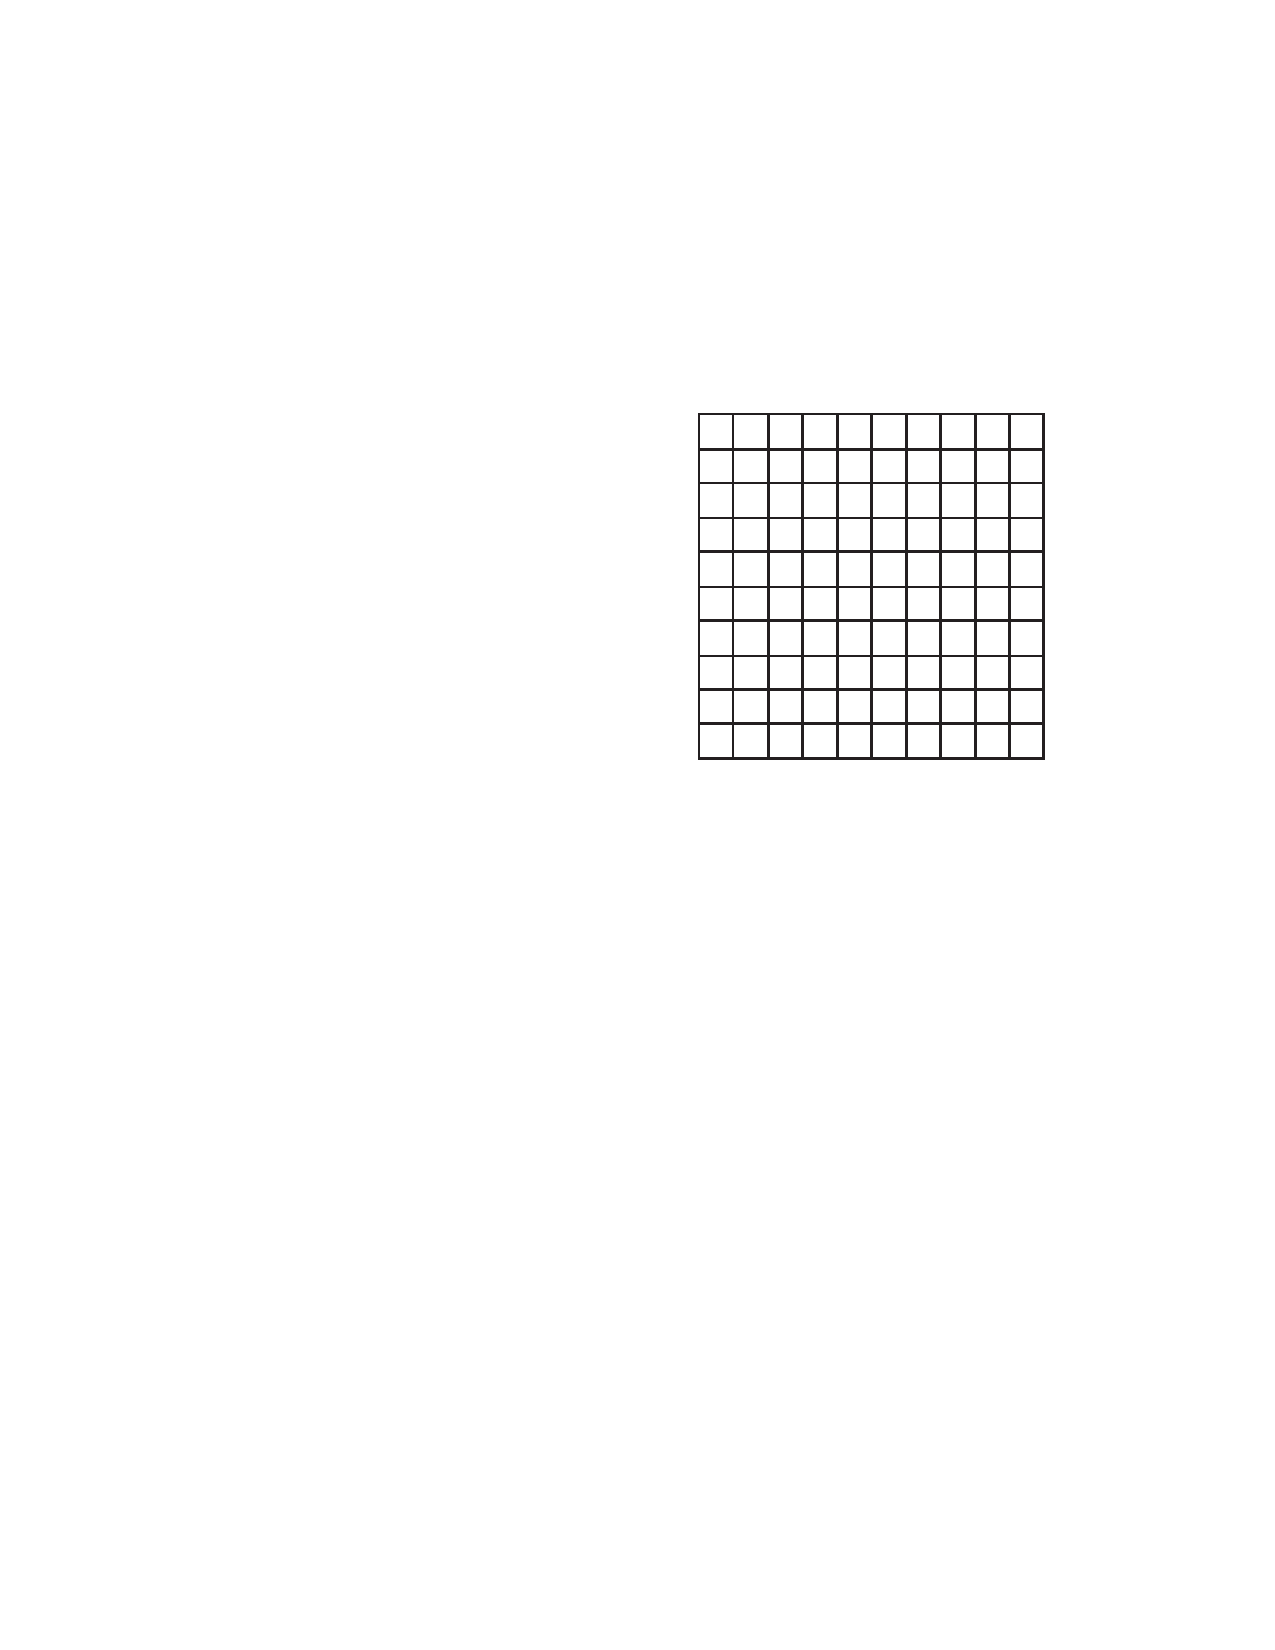
\includegraphics{../graphics/hundredthsGrid}\quad
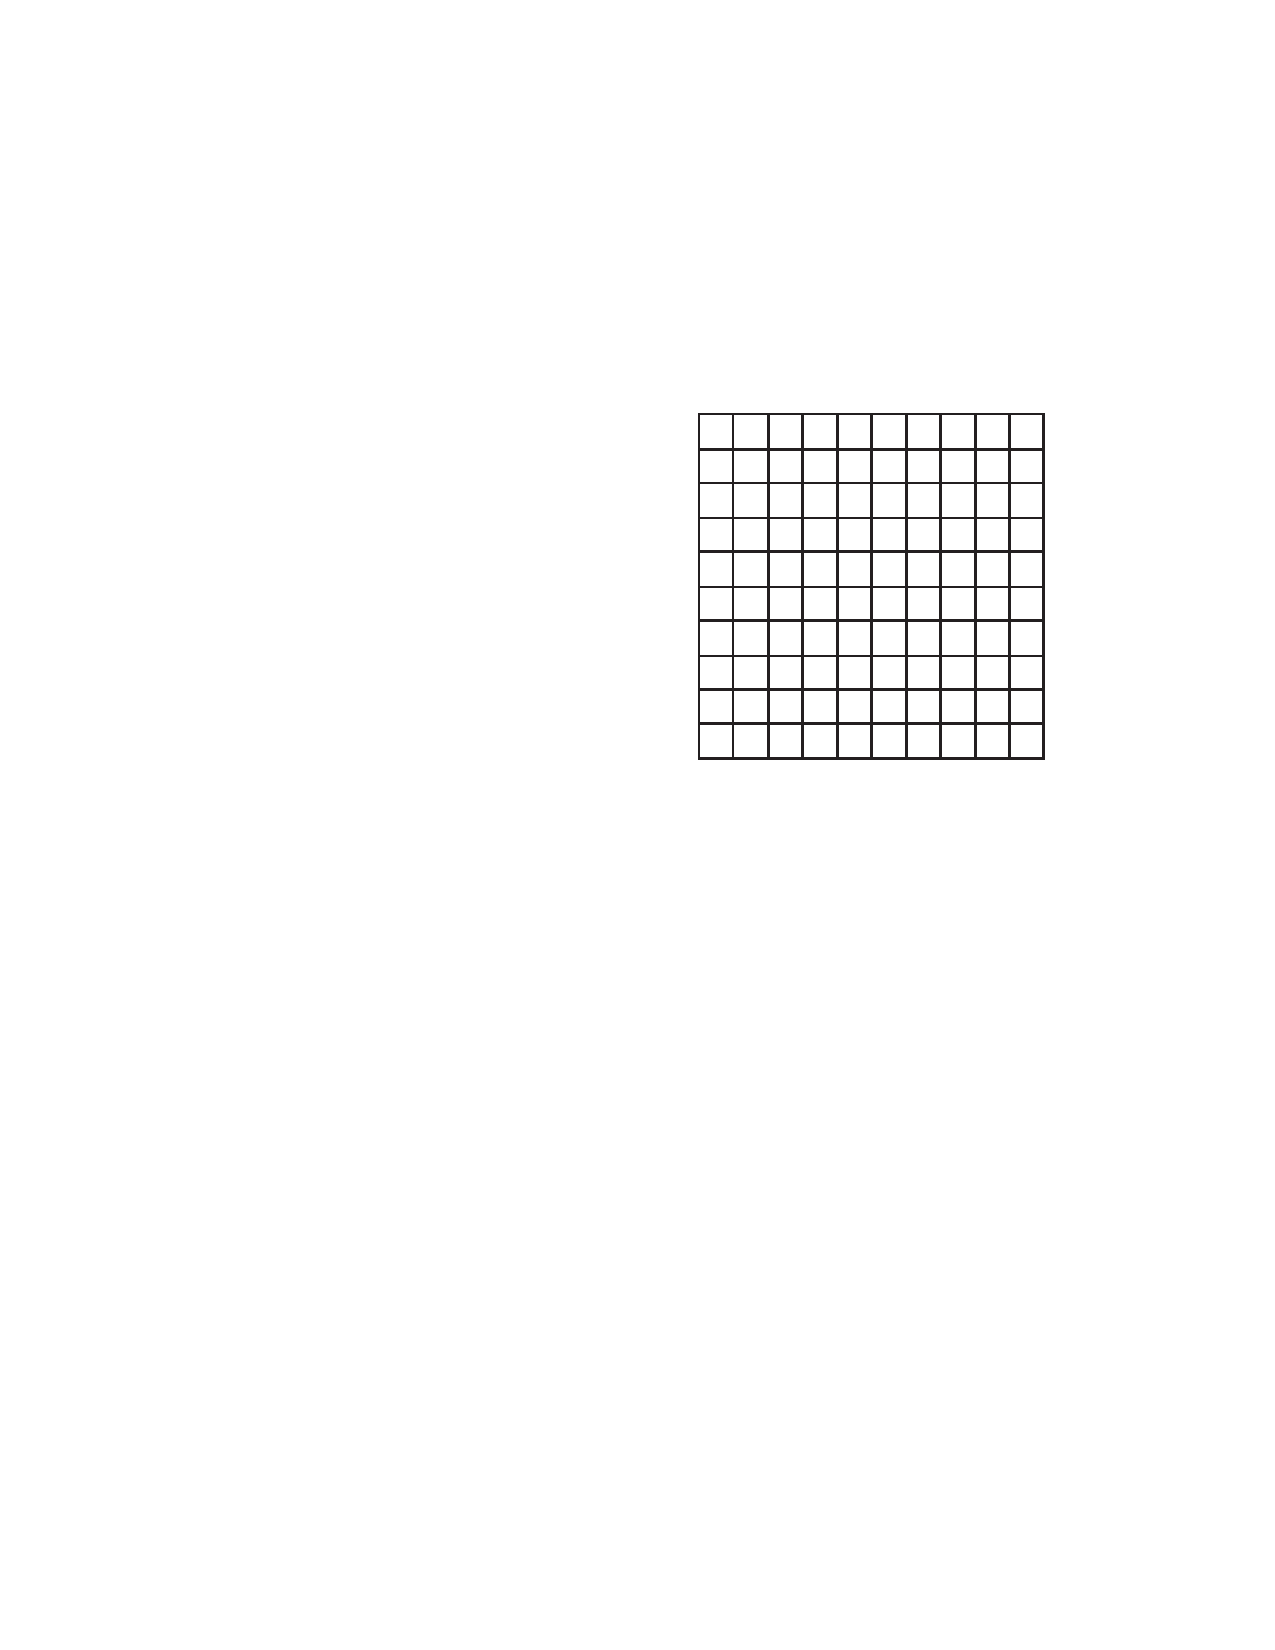
\includegraphics{../graphics/hundredthsGrid}
\end{fullwidth}

\end{prob}


